% !TeX root = ..//diffgeo_main.tex
\begin{hlem}[Existenz einer Glockenfunktion]
Sei $U \subseteq M$ offen, $p \in U$. Dann $\exists \varphi \in \mathcal{F}(M)$, s. d. 
\begin{enumerate}\label{Glockenfunktion}
\item$\operatorname{supp}\varphi\subseteq U$
\item$\varphi$ auf einer Umgebung $U' \subset U$ von $p$ ist
\end{enumerate}
\end{hlem}

\begin{figure}[H]
\centering 
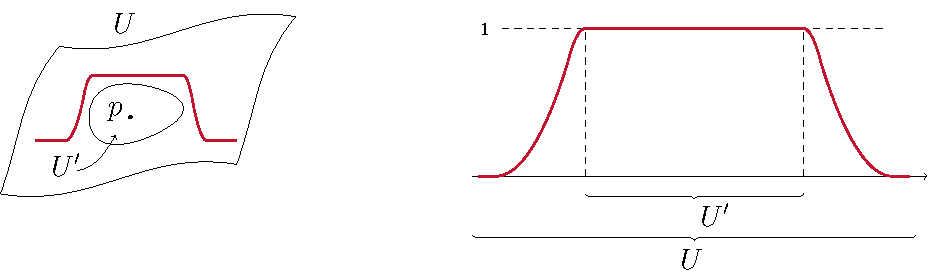
\includegraphics[scale=0.8]{figures/tikz/bump_function.pdf}
\caption{Visualisierung des Hilfslemmas  (\ref{Glockenfunktion}) \  ("bump function") }
\end{figure}

\begin{bew}
Sei $(x, U)$ eine Karte um $\varphi$, $\varepsilon > 0$, s. d. $B_{2\varepsilon}(x(p))\subset V\subset \R^n$ und wähle $\psi:\R^n\rightarrow\R$ mit 
\begin{align*}
\left.
\begin{array}{r}
\operatorname{supp}(\varphi)\subset B_{2\varepsilon}(x(p))\\
\varphi = 1 \text{ auf } B_\varepsilon
\end{array}
\right\} \text{ Resultat aus Analysis}\\
\end{align*}

Setze $\varphi(q) = \left\{
\begin{array}{l}
\psi(x(q))\text{ für }q\in U\\
0 \text{ sonst}
\end{array}
\right.$
\end{bew}

\begin{satz}[Eigenschaften des Tangentialraums]
Für $v\in T_p M$ gilt:
\begin{enumerate}
\item$v(\text{konstante Funktion}) = 0$
\item Falls $f = g$ in einer Umgebung von $p$, so gilt $v(f) = v(g)$
\end{enumerate}
"Lokalisierung von Tangentialvektoren"
\end{satz}

\begin{bew}[zu 2]
Wähle $\varphi$ wie im Hilfslemma, wobei $U$so gewählt ist, dass $\varphi f = \varphi g$ auf $U$ ist. Nun gilt:
\begin{align*}
v(\varphi f) &= v(\varphi)f(p) + \varphi(p)v(f)\\
&= v(\varphi)f(p) + v(f)\\
v(\varphi g) &= v(\varphi)g(p) + v(g)
\end{align*}
Dann folgt $v(\varphi f) = v(\varphi g) \Leftrightarrow v(f) = v(g)$.
\end{bew}

\begin{bew}[zu 1]
	$v(\lambda f) = \lambda v(f),\ \lambda \in \R,\ f\in \mathcal{F}(\R)$\\
	\textit{zz:} $v(\lambda) = 0$. Aufgrund von $v(\lambda) = \lambda v(1)$ genügt es zu zeigen, dess $v(1) = 0$. Dies folgt aus der Produktregel
	\begin{align*}
	v(1) = v(1*1) = 1v(1) + v(1)1 = 2v(1) \Rightarrow v(1) = 0
	\end{align*}
\end{bew}

